% !TEX encoding = UTF-8 Unicode
%!TeX TS-program = pdfLaTeX
%!TeX spellcheck = en-US
%!BIB TS-program = bibtex
% -*- coding: UTF-8; -*-
% vim: set fenc=utf-8
%
% public
% https://github.com/SpikeAI/pyTERtorch/tree/main/2022-09-30_BiolCybernetics
% https://www.zotero.org/groups/4776796/fastmotiondetection

% private
% https://framateam.org/spikeai/channels/2022-10_icip-bordeaux
% https://www.overleaf.com/project/630f9044c38e7a3cea81a7b2

%%%%%%%%%%%%%%%%%%%%%%%%%%%%%%%%%%%%%%%%%%%%%%%%%%%%%%%%%%%%%%%%%%
% 2022-09-30
% Learning heterogeneous delays in a layer of spiking neurons for fast motion detection
% Corresponding Author: Laurent Perrinet
% Biological Cybernetics
% a7f45f8e-87d6-4a30-ac7f-9f0c94e2592a   |  v.1.0
%%%%%%%%%%%%%%%%%%%%%%%%%%%%%%%%%%%%%%%%%%%%%%%%%%%%%%%%%%%%%%%%%%
%%%%%%%%%%%%%%%%%%%%%%%%%%%%%%%%%%%%%%%%%%%%%%%%%%%%%%%%%%%%%%%%%%
%Call for papers: Biological Cybernetics Special Issue: What can Computer Vision learn from Visual Neuroscience?
%
% https://www.springer.com/journal/422/updates/20421374
%
%Computer vision still struggles to solve many problems as quickly and accurately as our brain does, despite its tremendous progress using deep learning over the last decade. Current challenges include geometry understanding, dynamic scene understanding, few shot learning of novel objects, anomaly and counterfeit detection, stable reproduction of imaginary visuals, and more. The brain achieves all these on a low computational cost and power budget (i.e., tens of watts), whereas the state-of-the-art computer vision models require multiple graphics processors consuming kilowatts of power. Hence, new inspirations from the brain could make computer vision more efficient, robust, and capable of continuous learning and adaptation. Although visual neuroscience literature provides knowledge about neuronal selectivities and early processing of visual inputs, computational modelling of neuronal and network behaviours with some degree of biological constraints and characteristics is an important tool to address many of the challenges facing computer vision. With new neuroscientific insights about deep cortical vision processing using the latest stimulation and recording technologies, it is important that we strive to understand the underlying computations and learning mechanisms, so that artificial vision systems with similar efficiency can be developed. This special issue invites original research and review articles related to topics in biological vision that can potentially benefit computer vision systems. The following is a non-exhaustive list of topics in biological vision that can also benefit computer vision systems.
%
%● Active vision’s role in visual search, scene understanding, social interactions, etc.
%
%● Learning in the visual system. Learning in biology is continual, few-shot, and adversarially robust.
%
%● The roles of recurrent and top-down connections in the visual cortex.
%
%● Spike based spatio-temporal processing and its implications for neuromorphic vision.
%
%● Motion perception in dynamic environments.
%
%● Neural coding schemes in the visual system (e.g., sparse coding, predictive coding, and temporal coding.)
%
%● The roles of attention mechanisms in biological vision.
%%%%%%%%%%%%%%%%%%%%%%%%%%%%%%%%%%%%%%%%%%%%%%%%%%%%%%%%%%%%%%%%%%
%%%%%%%%%%%%%%%%%%%%%%%%%%%%%%%%%%%%%%%%%%%%%%%%%%%%%%%%%%%%%%%%%%
\newcommand{\Title}{
Learning heterogeneous delays in a layer of spiking neurons for fast motion detection
}
\newcommand{\ShortTitle}{
Learning heterogeneous delays of spiking neurons for motion detection
}
\newcommand{\FirstAG}{Antoine}
\newcommand{\LastAG}{Grimaldi}
\newcommand{\AuthorAG}{\FirstAG \LastAG}
\newcommand{\FirstLP}{Laurent U}
\newcommand{\LastLP}{Perrinet}
\newcommand{\AuthorLP}{\FirstLP \LastLP}
\newcommand{\EmailLP}{laurent.perrinet@univ-amu.fr}
\newcommand{\EmailAG}{antoine.grimaldi@univ-amu.fr}
\newcommand{\orcidLP}{0000-0002-9536-010X}
\newcommand{\orcidAG}{0000-0002-3107-4788}
\newcommand{\Department}{Institut de Neurosciences de la Timone}% (UMR 7289)}%
\newcommand{\Affiliation}{Aix Marseille Univ, CNRS}%
\newcommand{\Street}{27 boulevard Jean Moulin}%
\newcommand{\PostCode}{13005}%
\newcommand{\City}{Marseille}%
\newcommand{\Country}{France}%
\newcommand{\WebsiteLP}{https://laurentperrinet.github.io}%
\newcommand{\Abstract}{
The response of a biological neuron depends on the precise timing of afferent spikes. This temporal aspect of the neuronal code is essential in understanding information processing in neurobiology and applies particularly well to the output of neuromorphic hardware such as event-based cameras. However, most artificial neuronal models do not take advantage of this minute temporal dimension. Inspired by this neuroscientific observation, we develop a model for the efficient detection of temporal spiking motifs based on a layer of neurons with heterogeneous delays which we apply to the computer vision task of motion detection. Indeed, the variety of synaptic delays on the dendritic tree allows to synchronize synaptic inputs as they reach the basal dendritic tree. We show this can be formalized as a time-invariant logistic regression which can be trained using labeled data. We apply this model to solve the specific computer vision problem of motion detection, and demonstrate its application to synthetic naturalistic videos transformed into event streams similar to the output of event-based cameras. In particular, we quantify how the accuracy of the model can vary with the total computational load. This end-to-end event-driven computational brick could help improve the performance of future Spiking Neural Network (SNN) algorithms and their prospective use in neuromorphic chips.
}
\newcommand{\Keywords}{time code, event-based computations, spiking neural networks, motion detection, efficient coding, logistic regression
}
\newcommand{\Funding}{
This research was funded by the European Union ERA-NET CHIST-ERA 2018 research and innovation program under grant agreement N° ANR-19-CHR3-0008-03 (``\href{APROVIS3D}{http://aprovis3d.eu/}''). % Agence Nationale de la Recherche %HL and 
LP received funding from the ANR project  N° ANR-20-CE23-0021 ``\href{AgileNeuroBot}{https://laurentperrinet.github.io/grant/anr-anr/}''
% LP received funding 
and from A*Midex grant number AMX-21-RID-025
``\href{PolyChronies}{https://laurentperrinet.github.io/grant/polychronies/}''. 
%HL received funding from a University of Montreal Artificial Intelligence scholarship. 
%
}
\newcommand{\Acknowledgments}{
Thanks to Thomas Schatz, Rosa Cossart, Hugo Ladret, Camille Besnainou and Jean-Nicolas Jérémie for useful discussions prior to the elaboration of this work. %
\Funding %
%For the purpose of open access, the author has applied a CC BY public copyright licence to any Author Accepted Manuscript version arising from this submission. This research was funded, in whole or in part, by [Organisation name, Grant #]. 
A CC-BY public copyright license has been applied by the authors to the present document and will be applied to all subsequent versions up to the Author Accepted Manuscript arising from this submission, in accordance with the grant’s open access conditions. 
}
\newcommand{\DataAvailability}{
This works is made reproducible using the following tools. First the code reproducing all figures is available on~\href{ https://github.com/SpikeAI/pyTERtorch}{GitHub}. % todo: make a new repo

\noindent %The paper is available a an~\href{https://arxiv.org/abs/2205.03635}{arXiv preprint} with links to previous versions ands to the code. 
Find also the associated~\href{https://www.zotero.org/groups/4776796/fastmotiondetection}{zotero group} used to regroup relevant literature on the subject.

% public
% https://github.com/SpikeAI/pyTERtorch/tree/main/2022-09-30_BiolCybernetics
% https://www.zotero.org/groups/4776796/fastmotiondetection

% private
% https://framateam.org/spikeai/channels/2022-10_icip-bordeaux
% https://www.overleaf.com/project/630f9044c38e7a3cea81a7b2

%In this section, please provide details regarding where data supporting reported results can be found, including links to publicly archived datasets analyzed or generated during the study. Please refer to suggested Data Availability Statements in section ``MDPI Research Data Policies'' at \url{https://www.mdpi.com/ethics}. If the study did not report any data, you might add ``Not applicable'' here. Chen
}

%%%%%%%%%%%%%%%%%%%%%%%%%%%%%%%%%%%%%%%%%%%%%%%%%%%%%%%%%%%%%%%%%%%%%
% NOTATIONS
% Pixel world
\newcommand{\presynaddr}{a} % pre address
\newcommand{\postsynaddr}{n} % post address
\newcommand{\numevent}{N_{ev}} % total number of events
\newcommand{\presynaddrspace}{\mathcal{A}} %presynaptic address space
\newcommand{\postsynaddrspace}{\mathcal{B}} %postsynaptic address space
\newcommand{\Npol}{N_\text{p}} % number of polarity
\newcommand{\Nneuron}{N_\text{n}} % number of output neurons in the layer
\newcommand{\arank}{r} % address index
\newcommand{\bias}{b} % bias for the MLR model
\newcommand{\synapse}{\sigma} % synapse
\newcommand{\synapticweight}{w} % synaptic weight
\newcommand{\synapticdelay}{\delta} % synaptic delay
\newcommand{\ranksyn}{s} % synapse index
\newcommand{\Nsyn}{N_{s}} % total number of synapses
\newcommand{\activeweights}{\mathcal{W}} 
\newcommand{\timev}{t} % time
\newcommand{\polev}{p} % polarity
\newcommand{\event}{\epsilon} % event
\newcommand{\eventstream}{\xi} % stream of events
\newcommand{\TS}{S} % time surface
\newcommand{\neuron}{\mathbf{n}} % neuron in the SNN (defined by the spatial position and the channel)
\newcommand{\postneuron}{\mathbf{m}} % post synaptic neuron in the SNN (defined by the spatial position and the kernel)
\newcommand{\channel}{\mathbf{p}} % channel
\newcommand{\layer}{\mathbf{L}} % layer
\newcommand{\ms}{\si{\milli\second}}%
\newcommand{\us}{\si{\micro\second}}%
\newcommand{\timecontext}{T} % time context (cf HOTS) matrice gathering last event times
\newcommand{\current}{I} % post synaptic current
\newcommand{\volt}{u} % membrane potential
\newcommand{\volts}{V} % matrix of membrane potentials
\newcommand{\gain}{\gamma} % homeostatic gain
\newcommand{\simil}{\beta} % similarity value
\newcommand{\Nclass}{N_\text{class}} % number of classes for MLR:
\newcommand{\Nx}{N_\text{X}}
\newcommand{\Ny}{N_\text{Y}}
\newcommand{\Ntime}{N_\text{t}}
\newcommand{\kernel}{K} % convolution kernel
%\newcommand{\kernelind}{\mathbf{k}} % indice of the kernel
\newcommand{\kernelind}{k} % indice of the kernel
\newcommand{\Kx}{K_\text{x}}
\newcommand{\Ky}{K_\text{y}}
\newcommand{\Ktime}{K_\text{t}}
\newcommand{\classiflayer}{\mathbf{C}}
\newcommand{\class}{c} % class k of the MLR
\newcommand{\lrweights}{\theta} % matrix of MLR weights
\newcommand{\lrtrue}{y} % true value of the prediction for MLR
\newcommand{\loss}{J} % cost function for MLR
\newcommand{\softmax}{\sigma}
\newcommand{\actfreq}{f}
\newcommand{\decision}{\hat{y}}
\newcommand{\colorsec}{black}
\newcommand{\colorsubsec}{black}
\newcommand{\speed}{v}
\newcommand{\Nspeed}{N_v}
% Example definitions.
% --------------------
\def\x{{\mathbf x}}
\def\L{{\cal L}}
%%%%%%%%%%%%%%%%%%%%%%%%%%%%%%%%%%%%%%%%%%%%%%%%%%%%%%%%%%%%%%%%%%

%%%%%%%%%%%%%%%%%%%%%%%%%%%%%%%%%%%%%%%%%%%%%%%%%%%%%%%%%%%%%%%%%%%%%
%%                                                                 %%
%% Please do not use \input{...} to include other tex files.       %%
%% Submit your LaTeX manuscript as one .tex document.              %%
%%                                                                 %%
%% All additional figures and files should be attached             %%
%% separately and not embedded in the \TeX\ document itself.       %%
%%                                                                 %%
%%%%%%%%%%%%%%%%%%%%%%%%%%%%%%%%%%%%%%%%%%%%%%%%%%%%%%%%%%%%%%%%%%%%%

%%\documentclass[referee,sn-basic]{sn-jnl}% referee option is meant for double line spacing

%%=======================================================%%
%% to print line numbers in the margin use lineno option %%
%%=======================================================%%

%%\documentclass[lineno,sn-basic]{sn-jnl}% Basic Springer Nature Reference Style/Chemistry Reference Style

%%======================================================%%
%% to compile with pdflatex/xelatex use pdflatex option %%
%%======================================================%%

%%\documentclass[pdflatex,sn-basic]{sn-jnl}% Basic Springer Nature Reference Style/Chemistry Reference Style

%%\documentclass[sn-basic]{sn-jnl}% Basic Springer Nature Reference Style/Chemistry Reference Style
%%\documentclass[sn-mathphys]{sn-jnl}% Math and Physical Sciences Reference Style
%%\documentclass[sn-aps]{sn-jnl}% American Physical Society (APS) Reference Style
%%\documentclass[sn-vancouver]{sn-jnl}% Vancouver Reference Style
%%\documentclass[sn-apa]{sn-jnl}% APA Reference Style
%%\documentclass[sn-chicago]{sn-jnl}% Chicago-based Humanities Reference Style
%%\documentclass[sn-standardnature]{sn-jnl}% Standard Nature Portfolio Reference Style
\documentclass[default]{sn-jnl}% Default
%%\documentclass[default,iicol]{sn-jnl}% Default with double column layout
%%\documentclass[iicol]{sn-jnl}

\usepackage[T1]{fontenc}
%\usepackage{textcomp}
\usepackage[utf8]{inputenc}

%%%% Standard Packages
%%<additional latex packages if required can be included here>
%\usepackage[lofdepth,lotdepth,position=top]{subfig}
%\usepackage{tabularx}
%%%%

%%%%%=============================================================================%%%%
%%%%  Remarks: This template is provided to aid authors with the preparation
%%%%  of original research articles intended for submission to journals published 
%%%%  by Springer Nature. The guidance has been prepared in partnership with 
%%%%  production teams to conform to Springer Nature technical requirements. 
%%%%  Editorial and presentation requirements differ among journal portfolios and 
%%%%  research disciplines. You may find sections in this template are irrelevant 
%%%%  to your work and are empowered to omit any such section if allowed by the 
%%%%  journal you intend to submit to. The submission guidelines and policies 
%%%%  of the journal take precedence. A detailed User Manual is available in the 
%%%%  template package for technical guidance.
%%%%%=============================================================================%%%%

\jyear{2022}%

%% as per the requirement new theorem styles can be included as shown below
\theoremstyle{thmstyleone}%
\newtheorem{theorem}{Theorem}%  meant for continuous numbers
%%\newtheorem{theorem}{Theorem}[section]% meant for sectionwise numbers
%% optional argument [theorem] produces theorem numbering sequence instead of independent numbers for Proposition
\newtheorem{proposition}[theorem]{Proposition}% 
%%\newtheorem{proposition}{Proposition}% to get separate numbers for theorem and proposition etc.

\theoremstyle{thmstyletwo}%
\newtheorem{example}{Example}%
\newtheorem{remark}{Remark}%

\theoremstyle{thmstylethree}%
\newtheorem{definition}{Definition}%

\raggedbottom

\newcommand{\seeFig}[1]{see Fig.~\ref{fig:#1}}%{see Figure~\ref{fig:#1}}
%% The preceding line is only needed to identify funding in the first footnote. If that is unneeded, please comment it out.
%\usepackage{cite}
%\usepackage[usenames,dvipsnames]{xcolor} %The package starts from the basic facilities of the color package, and provides easy driver-independent access to several kinds of color tints, shades, tones, and mixes of arbitrary colors.
%\usepackage{tcolorbox} % define boxes that can be customed, has to be loaded after xcolor package
\usepackage{amsmath,amssymb,amsfonts} % amsmath and amssymb packages, useful for mathematical formulas and symbols
%%\usepackage{float} %allows me to use [H] with figures to insert figures in multicol env (poster)
%\usepackage{ulem} %The package provides an \ul (underline) command which will break over line ends; this technique may be used to replace \em (both in that form and as the \emph command), so as to make output look as if it comes from a typewrite. Caution: with this package, bibliography will make unbreakable and underlined journal titles
%\usepackage[switch]{lineno} % add line numbers
%\modulolinenumbers[5]
\usepackage{physics} %The  goal  of  this  package  is  to  make  typesetting  equations  for  physics  simpler,  faster,  and  more  human-readable.
%\usepackage{lineno} %Adds line numbers to selected paragraphs with reference possible through the LaTeX \ref and \pageref cross reference mechanism.
%\usepackage{hyperref} %The hyperref package is used to handle cross-referencing commands in LaTeX to produce hypertext links in the document
%\hypersetup{
%    colorlinks = false,
%    hidelinks
%    %linkbordercolor = {white},
%}
%\usepackage{array} %An extended implementation of the array and tabular environments which extends the options for column formats, and provides “programmable” format specifications.
%\usepackage{multicol} %Multicol defines a multicols environment which typesets text in multiple columns
%%\usepackage{wrapfig} %Allows figures or tables to have text wrapped around them. wrapfig is used when calling multicols
% \usepackage[position=top]{subfig} %The package provides support for the manipulation and reference of small or ‘sub’ figures and tables within a single figure or table environment. Linked to subfloat.
% for units
\usepackage{siunitx}%The siunitx package provides a  set  of  tools  for  authors  to  typeset  quantities  in  aconsistent  way.
\AtBeginDocument{\RenewCommandCopy\qty\SI}
\DeclareMathOperator*{\argmax}{arg\,max}
\DeclareMathOperator*{\argmin}{arg\,min}

%%%%%%%%%%%%%%%%%%%%%%%%%%%%%%%%%%%%%%%%%%%%%%%%%%%%%%%%%%%%%%%%%%
% a simpler annotation system:
\usepackage{soulutf8}
\usepackage{color}
\newcommand{\note}[1]{{\sethlcolor{yellow}\hl{#1}}}
%\newcommand{\note}[1]{}
%
\begin{document}
%%%-----------------------------------------------------------------
% Title.
% ------
\title[\ShortTitle]{\Title}
\artnote{This article is published as part of the Special Issue on "What can Computer Vision learn from Visual Neuroscience?"}
%
% Single address.
% ---------------
\author{\fnm{\FirstAG} \sur{\LastAG}}\email{\EmailAG}
\author{\fnm{\FirstLP} \sur{\LastLP}}\email{\EmailLP}
\affil{\orgdiv{\Department}, \orgname{\Affiliation}\\ \orgaddress{\street{\Street}, \city{\City}, \postcode{\PostCode}, \country{\Country}}}

%%==================================%%
%% sample for unstructured abstract %%
%%==================================%%

\abstract{
\Abstract
}

%\ninept
%
%\abstract{Abstract}
%
\keywords{\Keywords}
%
\maketitle
%%%%%%%%% BODY TEXT
\section{Introduction}
%%%-----------------------------------------------------------------
%%%-----------------------------------------------------------------
\label{sec:intro}
% >>>>>>>>>>> LuP is here <<<<<<<<<<<
%
\subsection{Recent challenges in machine learning and computer vision}
%%%-----------------------------------------------------------------
Machine learning, and computer vision in particular, have undergone a major transformation in modern times, transitioning from an active character in science fiction movies to become mainstream tools found in the smartphones in everyone's pocket. Less visible, yet crucial to our economy and security, these automated tools now dominate the range of services that equip virtually most sectors of our daily lives. This trend is profoundly pronounced in the field of medicine, as it provides practitioners with new diagnostic tools to treat people faster and more effectively. This particular example also illustrates some important challenges that these tools are increasingly facing. One of these is the sensitivity of deep-learning based algorithms to adversarial attacks, that is, the sensitivity of the models' output to minute changes in the input. This could raise important questions about the reliability of the results of any automated diagnostic model. More generally, these models do give an output for any possible input, but they lack an explanation as to why they produced it. This lack of explainability is a hindrance to the advancement of these methodologies, as well as to their acceptance for most safety-relevant tasks. Having said that, we may remember that these tools are inherited from theoretical models originally designed to understand the brain. While the first artificial neural networks were mainly applied to toy-like problems, they also offered a growing number of applications in machine learning and computer vision, but also more generally for task automation. In particular, convolutional neural networks are inspired by the feed-forward processing observed in the visual pathways of primates, and today they reach higher performances than humans for key image categorization challenges. One of the challenges of these models is to be able to scale them up for future applications, for example in autonomous driving. Indeed, in such applications, the input does not consist of a single image (say a few million pixels) but of a continuous stream of images from several cameras.

The challenges are numerous in such situations, and two major obstacles must be highlighted: the computational delay and the energy budget. First, most existing solutions are built incrementally from models built to process low definition images, such as Le Net for MNIST~\citep{lecun_gradient-based_1998}, then high definition images, such as VGG on ImageNet~\citep{simonyan_very_2015}. This has a cost and notably the fact that the computation time increases with the size of the image. This phenomenon has been mitigated by the increase in available computing power, notably thanks to the parallel processing implemented in GPU cards. However, the transition from images to videos, then to multiple cameras implies a further level in the change of scale in the amount of data processed. It also raises an issue that is often not addressed when it comes to image categorization, that is, of the right timing to take a decision. Indeed, in autonomous driving, an important task is to react as quickly as possible to a possible collision, for example when a pedestrian unexpectedly crosses the street. As such, future systems should always be able to give a response at any time, instead of having to wait for the pipeline to provide the correct answer. This online processing is also a feature of processing in biological systems and could be an important first contribution if we could translate these principles into future automated processes. %
Second, a major constraint for future systems is energy cost. As we have seen, fast computation time has been maintained for high-dimensional images, but at the cost of higher energy consumption. In addition, the need to solve increasingly complex tasks has required the construction of increasingly complex and deep architectures. As an example, the best performing model in the ImageNet challenge uses 2100 million parameters. Training the model typically consumes kilowatts of power and about 1 joule to infer a decision per single image. Less power-hungry solutions have emerged, such as Mobile Net~\citep{howard_searching_2019}, but they are not yet ready for practical use in autonomous cars, as the additional power consumption would be a significant percentage of the energy consumed by an electric car under standard conditions.

% The brain achieves all these on a low computational cost and power budget (i.e., tens of watts), whereas the state-of-the-art computer vision models require multiple graphics processors consuming kilowatts of power
Neuroscience could provide revolutionary answers to these two closely related problems. Indeed, the human brain has the remarkable property of being able to react at any time, while consuming a reasonable amount of energy, about tens of watts. This system is the result of millions of years of natural selection, and a striking difference between biological neural networks and artificial ones is the representation they use. CNNs, for example, represent information passing from one layer to another as tensors representing visual information densely over the visual topography, while representing different properties in different channels. These networks have been known to mimic many properties of biological systems~\citep{schrimpf_brain-score_2020}, yet, this score does not count rapidity or energy. On the other hand, information in a large majority of biological neural networks is represented as spikes, i.e. prototypical all-or-nothing events whose only parameters are their timing and the address of the neuron that emitted this spike~\citep{paugam-moisy_computing_2012}. Why spikes? It is not yet known why most biological systems have evolved to use this representation, but one major advantage seems to be some form of efficiency. In the human brain, each of the approximately 90 trillion nerve cells emits on average one spike per second which fan out to an average of 10000 synapses. Importantly, each neuron fires with great variability, and up to 300 spikes per second. Many attempts have been made to build artificial spiking neural networks (SNNs), and in particular to achieve the same performance as observed in classical CNNs with a lower energy budget. However, none of these networks has yet surpassed the state-of-the-art performances. Here, we will try to focus on one core property of spiking neurons, inspired by neurobiology to progress in this direction.
%
\subsection{What can neuroscience bring to computer vision?}% and the heterogeneous delays in spiking neurons} ~\citep{}
%%%-----------------------------------------------------------------
Let us first review some existing SNN models. A first motivation for these models was to understand biological observations at the different scales of the central nervous system. For example, the Hodgkin-Huxley model describes the dynamics of the membrane potential of a single nerve cell and specifically explains the role of the different voltage-dependent ion channels. It also explains how the model can produce a spike. Larger scale models introduce an simpler dynamics and an explicit spiking mechanism, for example in the Integrate-and-Fire model. It predicts the emergent states of a recurrently connected neural network~\citep{brunel_phase_2000}. Several models have increased the scale of the system to include more neurons, such as The Virtual Brain (TVB)~\citep{sanz_leon_virtual_2013}, which mixes different scales and includes SNNs with (analog) neural mass models. However, these methods are mainly descriptive with applications in neuroscience but few spiking neural models have had an application in computer vision. Another class of approaches have designed normative models of SNNs that aim to have applications in machine learning. One of these is the SpikeNet algorithm, which uses a purely temporal approach by encoding information using one spike per neuron~\citep{delorme_spikenet_1999}. Another type of SNN using precise spike timing attempts to determine the structure of the network in order to minimize a cost function. This was implemented in the SpikeProp algorithm~\citep{bohte_error-backpropagation_2002} and has been extanded in novel gradient-based methods. The surrogate gradient method is now widely used in methods that attempt to transfer performance from CNNs to SNNs~\citep{zenke_remarkable_2021}. However, the performance of SNNs is still lagging that of analog networks and the question of the advantage of using spikes in machine learning and computer vision remains open.

A new generation of algorithms has emerged with the advent of so-called silicon retinas, which mimics the output of the retina by representing visual information using spikes. %A novel emerging representation is that provided by event-based cameras, in which each pixel independently processes its input and emits an event for positive or negative increments of the log-luminance. 
The shift from the classical, dense representations to this sparse encoding of visual information offers a better analogy to neurobiology, but also offers more energy-efficient computations. It also allows using the precise timing of events. In the HOTS model for instance, the event stream induces spatio-temporal relationships between events which are represented by building ``time surfaces'', 2D images computed using the time difference to the last recorded events~\citep{lagorce_hots_2017}. In a recent study, we have introduced a SNN as a classification model applied to event-based streams using Multinomial Logistic Regression (MLR)~\citep{grimaldi_robust_2022} which extended the HOTS model. By transforming each event in the stream as a vectorial input, our MLR classifier was able to make a decision for every single event, that is, in an online fashion. We have demonstrated on several benchmark datasets that it provides with efficient computations, resulting in ultra-fast categorization. Additionally, we made a formal bridge between this event-based MLR and a SNN, demonstrating the bio-plausibility of this method and its possible integration to neuromorphic hardware. A serie of similar algorithms are applied to real-life applications such as optical flow~\citep{benosman_asynchronous_2012}, depth estimation~\citep{dardelet_event-by-event_2021}, or gesture recognition~\citep{maro_event-based_2020}. Recently, such an algorithm was used in the CASPR mission on the International Space Station, illustrating, given the stringent selection processes used by the space sector, that such algorithms have reached maturity for industry.

These computational results suggest that the temporal representation underlying processing in spiking neurons may be a key ingredient in the efficiency of the algorithms, but one may wonder how this can be supported by neurobiological data. In 1982, Abeles asked if the role of cortical neurons is whether to integrate synaptic inputs or rather to detect coincidences in temporal spiking motifs~\citep{abeles_role_1982}. While the first possibility favors the rate coding theory, the second highlights the function of temporal precision in the neural code. Since, numerous studies demonstrated the emergence of synchronicity in the activity within a neural population~\citep{riehle_spike_1997, davis_spontaneous_2021}, efficient encoding thanks to the use of spike latencies~\citep{perrinet_coding_2004, gollisch_rapid_2008} or precise timing in the auditory system~\citep{deweese_binary_2002, carr_circuit_1990}. All these findings, and more~\citep{bohte_evidence_2004}, highlight the importance of the temporal aspect of the neural code and suggest the existence of spatio-temporal spiking motifs in biological spike trains. In neuronal models, an efficient use or detection of these spatio-temporal motifs embedded in the spike train comes with the integration of heterogeneous delays~\citep{gutig_tempotron_2006, guise_bayesian_2014, zhang_supervised_2020}. Notably,~\citet{izhikevich_polychronization_2006} introduced the notion of the polychronous group as a repetitive motif of spikes defined by a subset of neurons with different, yet precise, relative spiking delays. This representation has a much greater information capacity in comparison to a firing-rate based neural coding approach through the variety of configurations and the possible coexistence of multiple superposed motifs.

This paper explores the possibility that prototypical spiking motifs may be a useful representation used in neurobiology and that we may transfer this hypothesis to neuromorphic algorithms. Our SNN model starts as a simple layer of leaky integrate-and-fire neurons whose connections are defined by a matrix of synaptic weights. Here, we propose to extend our model to a layer of spiking neurons which include heterogeneous delays in addition to weights. In particular, one afferent may be connected with multiple delays. Crucially, we will explicitly use the delay in the computational process. As a consequence, this extends our previous MLR model by encoding spiking motifs as spatio-temporal patterns. The objective in this model, by including the dimension of temporal delays, is to increase the representational capacities of the classifier. In the perspective of building energy-efficient algorithms, we will also titrate quantitatively the best trade-off between robustness and computation time when increasing the number of these heterogeneous delays. %
%
\subsection{Outline}
%%%-----------------------------------------------------------------
In this work, we study the emergence of spatio-temporal spiking motifs when training a single layer of spiking neurons on a semi-supervised classification task (\seeFig{motion_task}). The paper is organized as follows. We develop a theoretically defined SNN capable of learning heterogeneous delays from spiking motifs that we first evaluate on a synthetic event-based dataset. We first detail the methodology by defining the basic mechanism of spiking neurons that utilize heterogeneous delays. This will allow us to formalize the spiking neuron used to learn the model's parameters and test its effectiveness. We aim to apply this model to a realistic motion detection task which we will first define. Then, we will show how the model can be adapted to solve the motion detection task. In the results section, we will detail the emergent structure of the model solving the task and show in particular the similarities with neurobiological observations. We will also test the network with classical stimuli used in neuroscience, and in particular with frequency or contrast responses.  We will also study the efficiency of the motion detection mechanism and in particular its resilience to synaptic weight pruning. This will allow us to show how such a model can provide an efficient solution to the energy/accuracy trade-off.  Finally, we will conclude by highlighting the main contributions of this paper, while defining some limitations. This will open perspectives for future SNNs.  In particular, as neuromorphic devices are by design good candidates for integrating computations over time, we highlight the fact that this event-driven algorithm is perfectly fit to be transfered to this type of hardware.
%
\section{Methods}
\label{sec:methods}
%%%-----------------------------------------------------------------
%%%-----------------------------------------------------------------
Let us now formally define the spiking neural network (SNN) model with heterogeneous delays, as well as the task and how we will learn to solve it. First, we will define the model for the efficient detection of event-based motifs using a feed-forward layer of spiking neurons with heterogeneous delays. Our SNN model will be tested on a computationally relevant task of detecting motion detection from an event-based sensory input. By analogy with biological conditions, we will design a paradigm simulating eye movements where an input image is translated by a parameterized saccadic trajectory. Solving this task is, for example, useful in real-life situations to compensate for eye, head or body movements and to provide robust image categorization by stabilizing the image on the retina. The task is thus to guess the motion as accurately as possible (\seeFig{motion_task}) and we will describe a semi-supervised learning mechanism for weights and delays. To this end, we will extend the SNN model to be efficient for the resolution of the task by including spatio-temporal convolutional kernels. We will finally describe its implementation on conventional computers. 
%
\subsection{Detecting event-based motifs using spiking neurons with heterogeneous delays}% model as a Logistic Regression with a temporal convolution}
%%%-----------------------------------------------------------------
%
\begin{figure}%[t!]
    \centering
    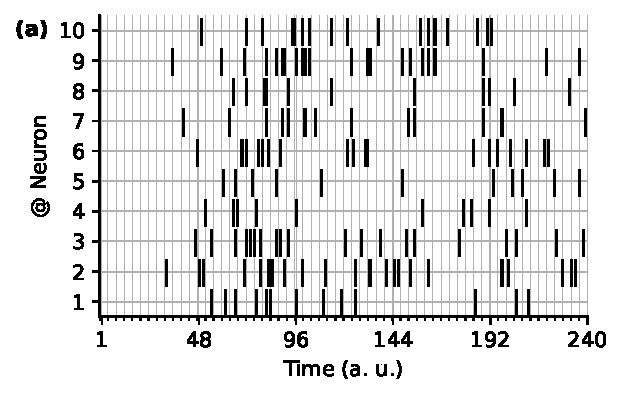
\includegraphics[width=0.490\linewidth]{figures/THC_1a_k.pdf}
    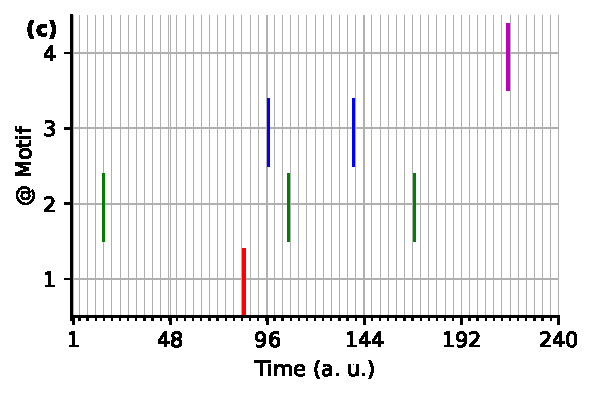
\includegraphics[width=0.490\linewidth]{figures/THC_1c.pdf}
    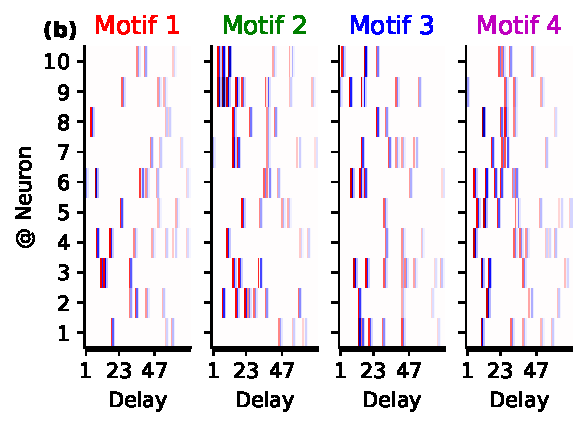
\includegraphics[width=0.490\linewidth]{figures/THC_1b.pdf}
    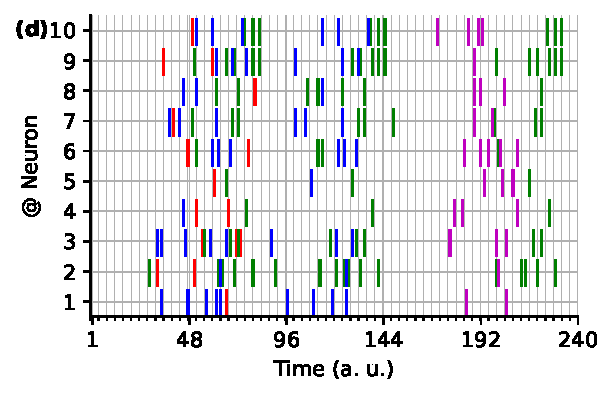
\includegraphics[width=0.490\linewidth]{figures/THC_1a.pdf}
	    \caption{Detecting event-based motifs using spiking neurons with heterogeneous delays. 
	    {\bf (a)}~Given a generic raster plot defined by a set of spikes occurring on specific addresses and at specific times, one may consider that this information consists of the repeated occurrence of groups of precise motifs of spikes that we call ``spiking motifs''. 
	    {\bf (b)}~We show some randomly drawn motifs, each identified at the top by a different color. To each neurons and $71$ different possible delays is assigned an evidence of activation (red) or deactivation (blue). 
	    {\bf (c)}~The activation in time of the different motifs is then used to define a generative model for drawing a raster plot on the multi-unit address space.
        % We will define a layer of neurons that will detect these PGs such that the addresses are the synapses of these neurons (which we therefore call here synapses).
	    Note that each afferent may be connected with multiple weights at different delays. The propagation of the afferent information through these delay may generate at each time step a synchronous motif on a subset of synapses. %These PG motifs were efficiently learned by a logistic regression.
	    % {\bf (c)}~The output of the model provides with the predicted probability of occurrence of each PG motif at any time, which may be used to generate a spike as a Bernoulli trial, providing in this particular case with an exact identification of PGs occurrences.
	    {\bf (d)}~Knowing the results of this detection, one may for illustration purposes highlight them by different colors in the raster plots, showing that in this synthetic examples, all spikes are now associated with a PG.  The original raster plot can be annotated with each identified spiking motif. 
	     }
    \label{fig:model}
\end{figure}
% 
\subsubsection{A generative model for raster plots}
%
As in a neurobiological recording or in the sensory signal representing the output of an event-based camera, any generic raster plot consists in a stream of \emph{spikes} (see Figure~\ref{fig:model}-(a)). This can be formalized as an ordered set $\event$ of addresses and timestamps $\{(\presynaddr_\arank, \timev_\arank)\}_{\arank \in [1,\numevent]}$ where $\numevent \in \mathbb{N} $ is the total number of events in the data stream and the rank $\arank$ is the index of each event. That event has a time of occurrence $\timev_\arank$  and an associated address $\presynaddr_\arank$ (which is typically in the form $(x_\arank, y_\arank, \polev_\arank)$ for event-based cameras). This defines an address space $\presynaddrspace$ which consists of the set of possible addresses. This can be the identified set of neurons in a neurobiological recording. For event-based cameras, it is denoted by $[1, \Nx]\times[1, \Ny] \times [1, \Npol] \subset \mathbb{N}^3$ where $(\Nx, \Ny)$ is the size of the sensor in pixels and $\Npol$ is the number of polarities ($\Npol=2$ for the ON and OFF polarities coded in event-based cameras). 

This raster plot is generated by spiking neurons which are defined on the one hand by the equations governing the evolution of its membrane potential dynamics on its soma and on the other hand by the characterization of the synaptic contacts on its dendritic tree, or on the sensory processes (such as the pixel on the sensor of a camera, or the photoreceptors in the retina). A classical characterization consists in detailing the synaptic weights of each synaptic contact on the dendritic tree, the so-called weight matrix. A more detailed description of these synaptic contacts reveals the added importance of heterogeneous delays, i.e., the precise timing from one afferent neuron's firing to its arrival in the soma, and how this changes the network's dynamics~\citep{izhikevich_polychronization_2006}. In that description, we can parameterize each neuron by the set of tuples defining both the weight and the delay of each synaptic contact. As a consequence, a set of input presynaptic spikes $\event$ will be processed by the dendrites defined by this synaptic set and notably by the respective delays, which will multiplex in time all events. 

Formally, let's define a layer of heterogeneous spiking neurons $\postsynaddr \in \postsynaddrspace$ by first describing how each neuron connects to presynaptic afferent from $\presynaddrspace$. In biology, a single cortical neuron has generally several thousands of synapses, and each synapse may be defined by its synaptic weight and its delay, that is, the time it takes for one spike to travel from the presynaptic neuron's soma to that of the postsynaptic neuron. A postsynaptic neuron $\postsynaddr \in \postsynaddrspace$ is then described by the synaptic weights connecting it to a presynaptic afferent from $\presynaddrspace$ but also by the set of possible delays. Note that a neuron may contact an afferent neuron with multiple different delays. For each neuron $\postsynaddr$, we thus define a set of $\Nsyn^\postsynaddr$ synapses, as  $\synapse^\postsynaddr = \{(\presynaddr^\postsynaddr_\ranksyn, \synapticweight^\postsynaddr_\ranksyn, \synapticdelay^\postsynaddr_\ranksyn)\}_{\ranksyn \in [1,\Nsyn^\postsynaddr]}$, where each synapse $\synapse^\postsynaddr_\ranksyn$ is associated to a weight $\synapticweight^\postsynaddr_\ranksyn$, a delay $\synapticdelay^\postsynaddr_\ranksyn$ and a presynaptic address $\presynaddr^\postsynaddr_\ranksyn$. This defines the full connectivity of the heterogeneous model. As a consequence, an event stream $\event_\presynaddrspace$ on the presynaptic address space is transformed by the synapse $\ranksyn$ of neuron $\postsynaddr$ into a new event stream $\event_{\presynaddrspace, \ranksyn}$ which is defined by 
$\{ (\presynaddr_\arank = 
 \presynaddr_\ranksyn^\postsynaddr, \timev=\timev_\arank + 
\synapticdelay_\ranksyn^\postsynaddr )_{ \arank \in [1,\numevent]\text{, }\ranksyn \in [1,\Nsyn^\postsynaddr]} )
\}$. This new stream of events \note{formaliser le multiplexage}
When post-synaptic neurons are activated on their soma by this spatio-temporal motif the discharge probability will increase, notably when these spikes converge on the soma in a synchronous manner. 

Taking the argument the other way around, one may form a generative model for generic raster plots. Indeed, any spike in the presynaptic address space is generated by sensory neurons (for instance photoreceptors in the retina, sensors in a CMOS chip) or by afferent spiking neurons. In the latter case, these are connected to the spiking cell by a set of weights and delays, whose structure is stable relatively to the coding timescale. When these connections are high and sparsely distributed, this firing will cause a specific temporal motif. Another example is given for the barn owl auditory system: As it hears the sound of a mouse, this sound will generate a specific spiking response in both ears, and specifically, the precise timing between the signal generated by the left relative to the right ear can be for instance used to determine the position of the prey~\citep{goodman_spike-timing-based_2010}. Overall, these examples show that raster plots may be considered as a mixture of the effects of different elementary causes, and that each event triggers a specific spatio-temporal motif. 
%
\subsubsection{Detecting spiking motifs}
%: Detection model

\note{ TODO: show why this formula implements a polychrony detector }
From the perspective of simulating such event-based computations on standard chips, it is useful to transform this sparse representation into a dense representation. As such, we may first write any event-based input as the boolean matrix $A \in \{0, 1 \}^\presynaddrspace$. In this simplified model, we will consider that heterogeneous delays are limited in range such that the synaptic set can be represented by the dense matrix $\kernel^\postsynaddr$ giving for each neuron $\postsynaddr$ the weights as a function of presynaptic address and delay: $\forall {\ranksyn \in [1,\Nsyn^\postsynaddr]}, \kernel^\postsynaddr(\presynaddr_\ranksyn^\postsynaddr, \synapticdelay_\ranksyn^\postsynaddr) = \synapticweight_\ranksyn^\postsynaddr$. 
The probability of firing of a neuron $a$ at a given time $t$ can be understood as a Bernoulli trial whose (only) parameter is a bias $p(t, a) \in [0, 1]$. Assuming that the presence of PGs conditions the probability on all efferents, the logit (inverse of the sigmoid) of this probability bias can be written as the sum of the logit of each of these factors, whose values are given by the corresponding weights. PGs may be activated independently at random times and  we write that $B(b, t)=1$ if $b$ is activated at $t$ (and else $B(b, t)=0$). We can thus write the probability bias as the accumulated evidence given these factors as 
\begin{equation*}
p(t, a) = \sigma\big(W_0 + \sum_{b, t} B(b, t) \cdot W_b(a, t-d) \big)  
\end{equation*}
where $\sigma$ is the sigmoid function. We will further assume that the weights are balanced (their mean is zero) and that $W_0$ is a bias such that $p_0=\sigma(W_0)$ is the average background firing rate. Conveniently, one can write this summation as a one-dimensional temporal convolution operator such that we may simply write
\begin{equation*}
p = \sigma(W_0 + B \ast W )
\end{equation*}
where  $p\in [ 0, 1]^{N\times T}$ and $B\in \{0, 1\}^{M\times T}$ is the raster plot corresponding to the temporal activation of the PGs. Finally, we obtain the raster plot $A\in \{0, 1\}^{N\times T}$ by drawing spikes using independent Bernoulli trials $A \sim \mathcal{B}(p)$. Note that, depending on the shape of the kernels, the generative model can model a Poisson process, generate rhythmic activity or more generally propagating waves. This formulation thus defines a simple generative model for raster plots as a combination of independent PGs. 
%
%Using this dense representation, the counting defined above becomes:
%\begin{equation*}
%\mathcal{C}^\postsynaddr(a,t)
%= \sum_{\presynaddr, \synapticdelay_\ranksyn^\postsynaddr} \kernel^\postsynaddr(\presynaddr_\ranksyn^\postsynaddr, \synapticdelay_\ranksyn^\postsynaddr) \cdot A(\presynaddr, \timev-\synapticdelay_\ranksyn^\postsynaddr)
%\end{equation*}
%%
%This shows that $\mathcal{C}^\postsynaddr$ is a temporal convolution of the dense representation of the event stream with the dense kernels formed by the set of synapses:  $\mathcal{C}^\postsynaddr = \kernel^\postsynaddr \ast A$.
%This well-known computation defines a time-invariant, differentiable measure which is very efficiently implemented for GPUs and which we will use for learning the classification of different motifs in the event stream.
%%
%
%\note{formalize the following:}
%More generally, every cause may be considered as occurring independently and one might write the generative model for the generation of the presynaptic events as:
%
%
%Using this formalization, one might now deduce an optimal algorithm for the detection of such temporal motifs.
%
%
%By discretization of time (with here an arbitrary unitary time unit), we can also define the dendrite as a matrix giving the weight corresponding to the different delays $d \in [0, D]$ (where $D$ is the maximum delay) on different pre-synaptic addresses $a \in [1, N]$ defining the list of the $N$ dendrites. We will denote as $W(a, d)$ these weights.
%
%
%Following the observations of~\citet{izhikevich_polychronization_2006}, let us assume that such precise discharge motif defines a polychronous group (PG). Assuming that we know there exists $M$ such groups, we will define as $b \in [1, M]$ the address of a PG and as $W_b$ the corresponding weight matrices. This allows then to derive a generative model for raster plots (see Figure~\ref{fig:model}-(b)).




%\subsubsection{Implementation using spiking neurons with heterogeneous delays}
%
The activation function of our spiking neural is a softmax function implementing a form of  Multinomial Logistic Regression (MLR)~\citep{grimaldi_robust_2022}, in analogy to a spiking Winner-Take-All network~\citep{nessler_bayesian_2013}. 
%It transforms this list of weights into a probability with the following formula:
%$
%Pr(k=\postsynaddr \; \vert \; \timev) =
%\frac 1 Z
%{\exp  (\mathcal{C}^\postsynaddr(\timev) +\bias^\postsynaddr) }
%$ 
%where $\mathcal{C}^\postsynaddr(\timev) = \sum
%\activeweights^\postsynaddr(t)
%$ is the sum of the synaptic weights and $\bias^\postsynaddr$ is the bias linked to neuron $\postsynaddr$. 
%In particular, we expect that some specific motifs may become tightly synchronized as they reach the basal dendritic tree, leading to a high postsynaptic activity which makes it progressively more likely to generate an output spike.
%%
%
\note{say that it is effortless in biology but difficult on conventional computers}
In our MLR model with $\Nclass=\Nspeed$ classes, a probability value is predicted for each event at address $\presynaddr_\arank$ and at time $\timev_\arank$ as a softmax function of the linear combination of the list of events on the basal dendrite of a neuron $\postsynaddr$ in association to a specific class. The linear combination can be defined by a set of synapses $\synapse^\postsynaddr$ as described in the heterogeneous delays model. 
%
\subsubsection{Performance on synthetic data}
%
\begin{figure}%[t!]
    \centering
    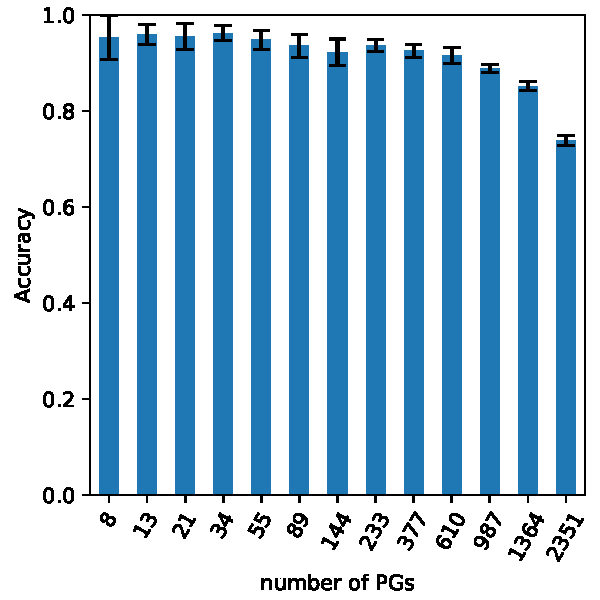
\includegraphics[width=0.490\linewidth]{figures/THC_N_PGs.pdf}
    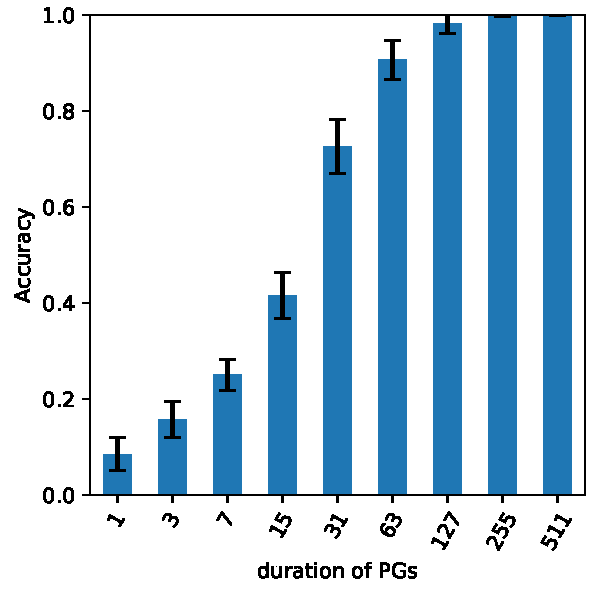
\includegraphics[width=0.490\linewidth]{figures/THC_N_PG_time.pdf}
	    \caption{Detecting event-based motifs using spiking neurons with heterogeneous delays. 
	    {\bf (a)}~Accuracy of PG detection as a function of the number $M$ of kernels.
	    {\bf (b)}~Accuracy of PG detection as a function of the temporal depth $D$ of kernels among $M=144$ kernels.
	    	     }
    \label{fig:model_results}
\end{figure}
% 
This generative model defined above allows to determine this inference model for guessing sources $B$ when observing a raster plot $A$. This assumes that we know the PGs as defined by the $W_b$ matrices. The underlying metric is the binary cross-entropy, as used in the logistic regression model. In particular, if we consider PG kernels with similar decreasing exponential time profile, we can prove that this is similar to the method of~\citet{berens_fast_2012}. In our specific case, the difference is that the regression is performed in both dendritic and delay space by extending the summation using a temporal convolution operator. Using this forward model, it is possible to estimate the logit (inverse of a sigmoid) $\hat{B}(b, t)$ for the presence of a PG of address $b$ and at time $t$ by using the transpose convolution operator. It thus comes that when observing $A$, then one may infer $\hat{B} = A \ast W^T$ and select the most activated items. 

To quantify the efficiency of this operation, we generated $M=55$ synthetic PGs as random independent kernels over $128$ presynaptic inputs and $D=127$ possible delays. We drew random independent instances of $B$ with a length of $T=1000$ time steps and with on average $2.0$ occurrences each. This allowed us to generate raster plots which we use to infer $\hat{B}$. We compute the accuracy as the rate of true positive detections (both for inferring the address and its exact timing) and observe on average $\approx 98\%$ correct detections. We further extended this result by showing how the accuracy would evolve as a function of the number of simultaneous PGs, while keeping the same frequency of occurrence. We show in Figure~\ref{fig:model_results}~(a) that the accuracy of finding the right PG is still above $80\%$ accuracy with more than $1364$ overlapping PGs. Moreover, we show in Figure~\ref{fig:model_results}~(b) that (with $M=55$ PGs fixed) the accuracy increases notably as the temporal depth $D$ of the PG kernel increased, demonstrating quantitatively the potential of heterogeneous delays. These results were obtained while assuming that we know $W$. However, this is in general not the case, for instance when observing the raster plot of a population of neurons. In the following, we will define a generic visual task and determine a learning algorithm to solve it. %Inspired by the k-means algorithm, it is possible to devise a self-supervised learning algorithm. Our preliminary results show that it is possible to retrieve PGs embedded in the data, yet that further analysis is necessary to improve the convergence of the algorithm. In particular, it seems promising to use a sparseness constraint in the inference mechanism such as to remove spurious correlations in the inference.
    
\subsection{Task definition: fast motion detection}
%%%-----------------------------------------------------------------
Let us now define a procedure of animating of natural scene by virtual eye-movements  similar to that which was used in neurobiological~\citep{vinje_sparse_2000, baudot_animation_2013} and computational neuroscience~\citep{kremkow_push-pull_2016} studies. First, let's define a trajectory inspired by the biological movements of the eyes. Indeed, these movements allow us to dynamically actuate the center of vision, or gaze, in the field of vision. In animals with a fovea, this is particularly useful as it allows to move the area with the highest density of photoreceptors in the environment, for example at a point of interest. For example, saccades are rapid movements of the eyeball that reposition the center of vision. In humans, these are very frequent (on average one every 3 per second~\citep{dandekar_neural_2012}). They are produced very rapidly (about $80~\ms$) and display a whole range of speeds. At a more microscopic scale, the human gaze moves with an incessant drift similar to a Brownian-like trajectory~\citep{poletti_head-eye_2015}. To maintain the full generality of the task, we will define eye movements using a form of random walk~\citep{engbert_integrated_2011}. This approach first defines a finite set of possible 2D motions in polar coordinates. Based on the distribution of biological motions, we simplified it by selecting a set of eye movements as the Cartesian product of % N-V-phi
$8$ linearly spaced motion directions and %N-Y-velocity=
$7$ different velocities (see inset of \seeFig{motion_task}-(a)). Note that the velocities are sampled on a geometric scale between $1/4$ and $4$. Next, we define one trajectory of gaze as segments whose duration is drawn from a Poisson distribution with an average block length of $20~\ms$, similarly to a Lévy flight~\citep[p. 289]{mandelbrot_fractal_1982}. Finally, the trajectory is integrated by assuming first that velocities are uniformly and independently sampled from the set of different motion-sets and second that motion is uniform during a time segment. The resulting instances yield trajectories qualitatively similar to those observed for human eye movements (\seeFig{motion_task}-(a)). 

%%%-----------------------------------------------------------------
%: fig:motion_task
%%%-----------------------------------------------------------------
\begin{figure}%[h!]%[ht!]
    \centering
    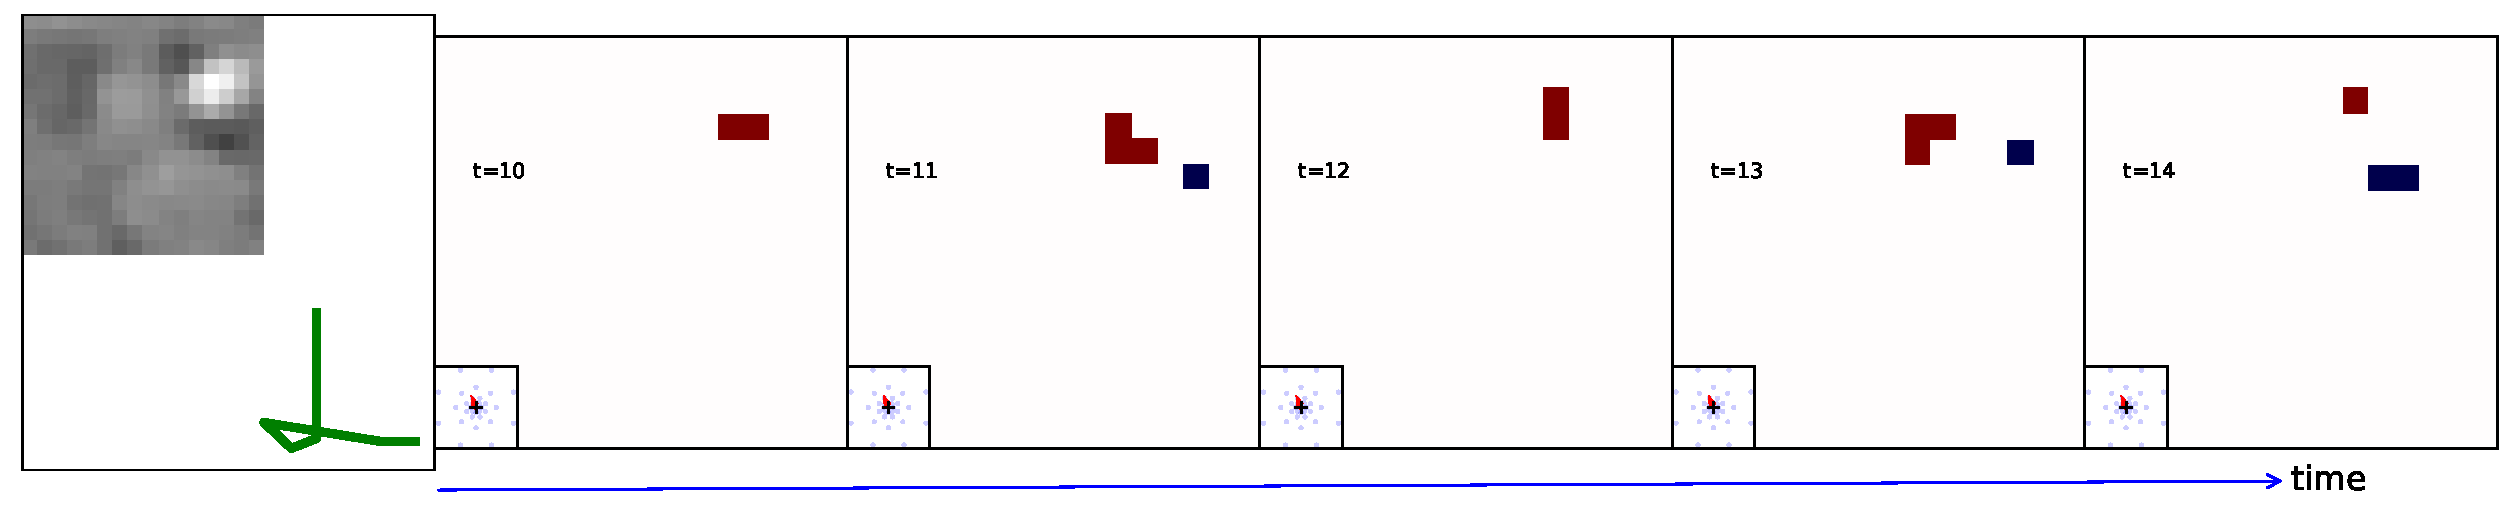
\includegraphics[width=0.95\linewidth]{figures/motion_task.pdf}
    \caption{
    {\bf Motion detection task.} {\bf (a)} We use large-scale natural images ($512\times512$) in which an aperture ($128\times128$) extracts a sub-image image in the axis of view (the image on the left) such as to reproduce the effect of displacing the eye. To mimic the effect of a saccadic-like eye movement, the axis of view moves following a step-like random walk, and we show here on example path of the trajectory as a green line ($200$ time steps). {\bf (b)} Recording the dynamics of the sub-image as a function of time, it generates a naturalistic movie which may be transformed to an event-based representation. Mimicking the retina, this representation codes for proportional increments or decrements of the luminance in the image, respectively ON (in red) and OFF (in blue) events. This will constitute the input to the SNN.}
    \label{fig:motion_task}
\end{figure}
%%%-----------------------------------------------------------------
Once these eye movement trajectories are generated, we can apply them to a visual scene. For this purpose, we selected a database of 10 natural grayscale images that are commonly used to study the statistics of natural images~\citep{olshausen_emergence_1996}. Note that these are pre-processed to equalize the energy in each frequency band (i.e., whitened). This process is known to occur as early as the retino-thalamic pathway~\citep{dan_efficient_1996}. These images are $512 \times 512$ in size and we will extract sub-images of size $128 \times 128$ which will be positioned around the center of the gaze at each time step (\seeFig{motion_task}-(b)). We will discretize the time in $1~\ms$ bins and produce movies of duration N-T = $250~\ms$. To avoid border effects, we will position a draw of the complete trajectory at random in the image space so that the sub-image is translated using the position given by the trajectory at each time step. The translation is computed using a coordinate roll in the horizontal and vertical dimensions, followed by a sub-pixel translation defined in Fourier space~\citep{perrinet_sparse_2015}. Note that the magnitude of the displacement is relative to the time bin, and we have defined the velocity such that a velocity of $V=1$ corresponds to a motion of one pixel per frame (i.e., per time bin).

\note{ TODO: formula / say it is driven by image gradients / give scaling rules }
To transform each movie into events, we compute a gradient image (initialized at zero) by adding the gradient of the pixels' intensity over two successive frames. If, on a specific pixel at that specific timestamp, the absolute value of this gradient exceeds a threshold, an event is generated. The event has either an OFF or ON polarity, respectively whether the gradient is negative or positive. This signed threshold value is then subtracted from the residual gradient image. When applied to the whole movie, the event stream is as a consequence similar to the output of a neuromorphic camera~\citep{rasetto_challenges_2022}, that is, a list of events defined by $x_\arank$ and $y_\arank$ (their position on the pixel grid), their polarity $\polev_\arank$ (ON or OFF) and time $\timev_\arank$  (\seeFig{motion_task}-(c)). The goal here is to infer the correct motion solely by observing these events. 
This sensory signal representing the output of this event-based camera forms a discrete stream of events, $\event$ as defined above.   
Each event has an associated address, which is typically in the form $\presynaddr_\arank=(x_\arank, y_\arank, \polev_\arank)$. This defines a presynaptic address space $\presynaddrspace = [1, \Nx]\times[1, \Ny] \times [1, \Npol] \subset \mathbb{N}^3$ where $(\Nx, \Ny)$ is the size of the sensor in pixels and $\Npol$ is the number of polarities  ($\Npol=2$ for ON and OFF polarities). 
\note{ the task is full-field rigid translations, the model resolves it locally (analogy to the input from V1 to MT) }
%
\subsection{Extension as 3D convolutions for motion detection}
%%%-----------------------------------------------------------------
%
Now that our motion detection task is defined in visual space, we can extend the convolution-based detection model to a 3D convolution so that the resulting model would also benefit from spatial invariance. The use of spatio-temporal filters on an event stream has improved the performance of CNNs for an action recognition task by~\citet{ghosh_spatiotemporal_2019} and here we will use a similar strategy, but focus on using an event-based representation.
For this purpose, we design 3D kernels of shape $(\Kx, \Ky, \Ktime) = (9, 9, 11)$, representing the two spatial dimensions and the range of time delays, respectively.
The computations are performed on the spatio-temporal windows that are defined by the kernels and are "moving" around the events, i.e. the spatial center of the spatio-temporal window around the current event $\epsilon_\arank$. Note that to remain within the framework of a causal calculation, the kernels are shifted in time such that only past information gives an answer at the present time.
%
The output of the MLR model corresponds to an event with the highest probability class, keeping the same timing as the input event. It is important to note that we include the prior knowledge that the event-based input is spatio-temporally clustered and that these clusters are sparse. Therefore, we will only select a given proportion of the most active cells, which we set here to $.01\%$ of all output voxels. This threshold was found using validation and future work should automate how this may be determined for various datasets. Given a stimulus input, the model thus yields a spike output in the postsynaptic address space.

%
Since the model is fully differentiable, we can now implement a semi-supervised learning rule. The loss function of the MLR model is the binary cross-entropy on the output of the classification layer and can be extended to space-time convolutions. Supervision was implemented using the input binary events as defined above and the labels as the desired output. The labels were defined at each time point as a one-shot encoding of the current motion in the channel corresponding to the current motion for all positions. As in this semi-supervised context, the label is known, but the timing is not, we used a selection of the temporal support in an unsupervised manner. It is important to note that we weighted the cost function by considering only active cells, such that the error is only back propagated to the spatial locations of these most active cells. This is reminiscent of previous methods solving this problem using a Winner-Takes-All mechanism~\citep{masquelier_unsupervised_2007}. Simulations are performed with the PyTorch library using gradient descent with Adam (for $2^{12}$ movies and a learning rate of $10^{-5}$). We tested the effect of different parameters on a validation set to quantify the role of each parameter.

%
Finally, the output of the MLR model is an event-based representation predicting at each position and at each time the probability of each motion. Such an output gives a form of optical flow that can be exploited for non-rigid motions, but we have defined here, for simplicity, an evaluation method that applies to our task with a full field motion. We have shown above that when different independent observations (here, the estimated motion at different spatial locations) are recognized as having a common cause (here, the rigid motion of the image), then an optimal estimate of the logit of this probability is the sum of the logits of the independent probabilities. By taking the logit of the probability of the output given by the model, we can therefore calculate the probability of the output. This allows one to calculate the accuracy (as the percentage of times the motion is accurately predicted) or the squared error % $|| \speed - ||^2$ 
of the velocity estimate given by the average estimate. 
%$\hat{\speed} = \sum_{\class} \speed_\class \cdot Pr(\class \vert image)$ 
These calculations are performed on a different input dataset than the one used in the training or validation steps. These metrics will be useful to compare our methods with other methods on our defined task.  The complete code to reproduce the results of this paper is available at \url{https://github.com/SpikeAI/pyTERtorch}.  
%
\section{Results}
\label{sec:results}
%%%-----------------------------------------------------------------
%: fig:kernels
%%%-----------------------------------------------------------------
\subsection{Kernels learned for motion detection}
%%%-----------------------------------------------------------------
\begin{figure*}[ht!]
    {\centering
    %\vspace{-3cm}
    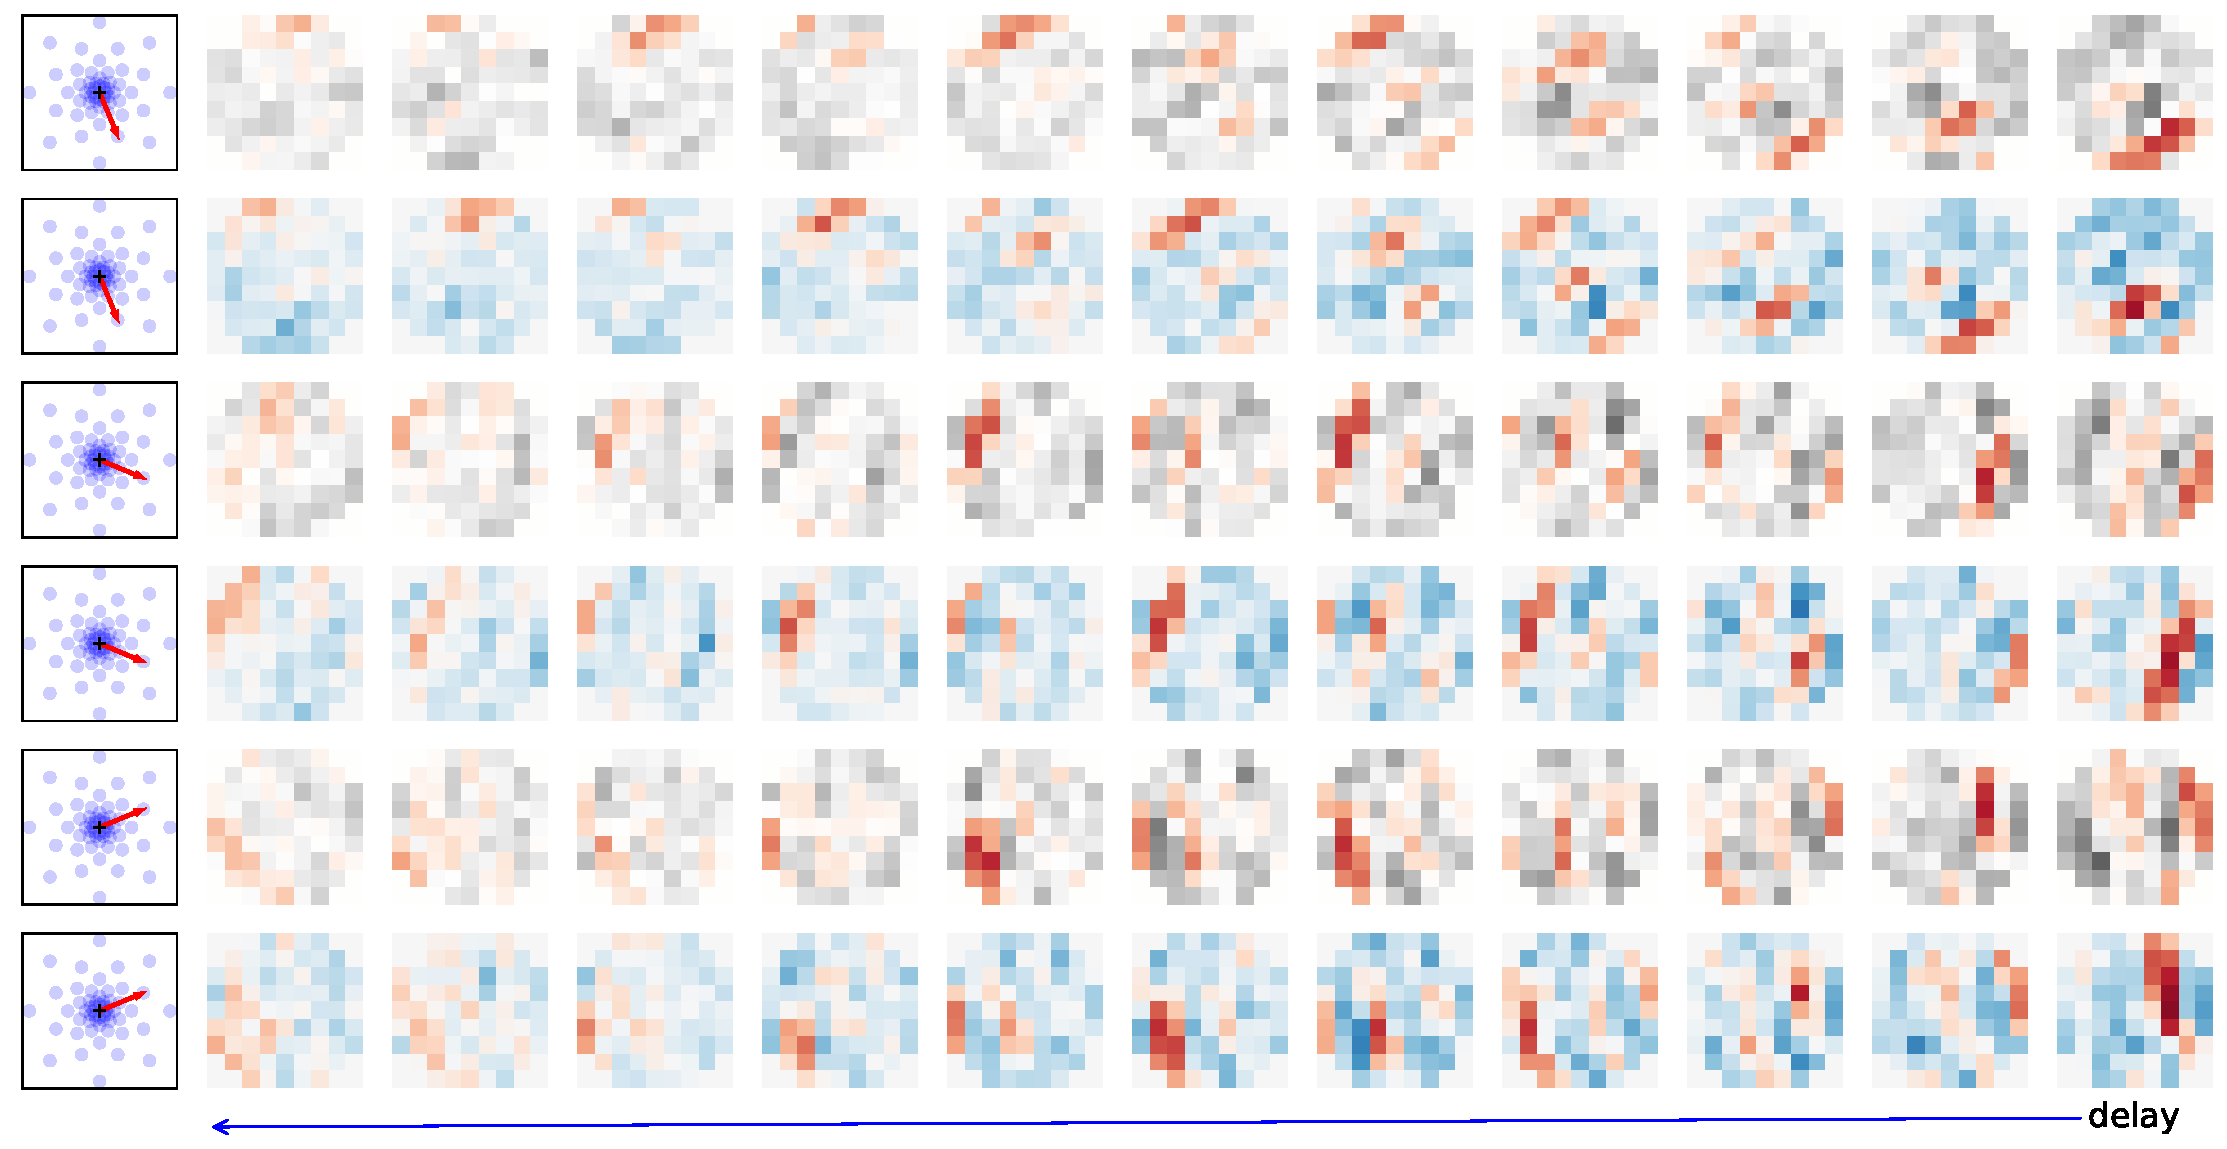
\includegraphics[width=\linewidth]{figures/motion_kernels.pdf}
    }
    %\vspace{-.5cm}
    \caption{
    	Representation of the weights for $3$ of the $32$ different learned kernels of the model. Each pair of line correspond to the OFF and ON polarities respectively, with excitatory weights in warm colors. Delays are represented in the horizontal axis from right (zero delay) to the left (delay of $11$ steps). Because of the symmetry observed between the ON and OFF event streams, we observed that kernels are very similar for the ON polarities. These weights are associated to a specific delay on the \textit{delays} axis and to a presynaptic address defined on the two other axes. %	For the sake of clarity, the values in range $[-0.05, 0.05]$ are not shown. 
	Different kernels are selective to the different motion directions and we observe some level of orientation selectivity, where ON and OFF subfields organized in a push-pull organization. 
%        One sees positive (excitatory) coefficients for the specific direction of motion but also negative (inhibitory) coefficients for other directions.
	}
    \label{fig:kernels}
\end{figure*} 
%
%
After training our model, we first analyze the weights learned for the different neurons (\seeFig{kernels}). 
We first observed a high dependence between the weights reaching the ON polarities and that reaching the OFF polarities. In particular, whenever a weight for a given position and delay is positive for one polarity, it will be negative in the other. This property comes from the way the events are generated and that the luminance can not at the same time increase and decrease. %ith the negative weights, one can observe an anti-selectivity for directions that do not correspond to the motion to which the kernel is selective to. 
We also observe that these cells show an orientation selectivity, similar to that observe in MT neurons~\citep{deangelis_functional_1999}. Interestingly, the relative organization of the receptive fields in quadrature of phase follows a push-pull organization predicted by~\citet{kremkow_push-pull_2016} to explain neurophysiological results~\citep{baudot_animation_2013}.  
Focusing on the positive weights, a strong selectivity is observed along specific axes of motion for each of the different kernels. These directions can be easily associated to the direction of motion controlled in the natural images. For instance, the first kernel shows a strong selectivity to horizontal motion directions.
%
%This qualitative look at the 3D kernels allows the reader to infer for the $8$ different motion directions used to generate our synthetic event streams.

If one focuses on the interpretation of these kernels in terms of spatio-temporal motifs embedded in the event stream, it can lead to interesting outcomes. In~\citep{grimaldi_robust_2022}, a link between event-based MLR training and Hebbian learning is drawn, allowing to say that the present model will learn its weights according to a presynaptic activity associated to the different motion directions. Each neuron becomes selective to a specific motion direction through the learning of an associated prototypical spatio-temporal spike motif. Each voxel in the 3D kernels defines a specific timestamp and a specific address. Consequently, our model is able to detect precise spatio-temporal motifs embedded in the spike train and associated to the different motion directions. The cone shape for the positive weights distribution highlights a loss of precision for longer delays, i.e. events away in the past. For the directions not coherent to the class of a training sample, an anti-Hebbian learning is also observed through the negative weights in the kernels of Figure~\ref{fig:kernels}. 

%
\note{kernel size has to be adapted to the characteristics of motion see Samonds %~\citep{samonds}
say that we have tested }
\note{tester la meme expe faite par baudot et modelisée par kremkow en montrant des raster plots du modele avec NI versus Gratings }

%%%-----------------------------------------------------------------
%
\subsection{Testing with natural-like textures}
%%%-----------------------------------------------------------------
To test our model, we will quantify its ability to categorize different motions. Before applying the model on natural images, we will first test the model on simpler, parameterized stimuli. In that order, we use a set of synthetic visual stimuli, \textit{Motion Clouds}~\citep{leon_motion_2012} which are natural-like random textures for which we can control for velocity, among other parameters (\seeFig{motion_clouds})~\citep{vacher_bayesian_2018}. In particular, we will set the spatial size and duration similarly to the motion task defined above.
This procedure defines a set of textures with different spatial properties and different motions $\va{v}_k$ with  $1 \le k \le \Nclass$ and $\Nclass=8$ defined by a constant speed and linearly spaced directions $
\speed_\kernelind = 
  ( 
    \speed \cdot \cos(2\pi\cdot \frac{\kernelind}{\Nspeed}),
    \speed \cdot \sin(2\pi\cdot \frac{\kernelind}{\Nspeed})
  )
$.
For any given velocity, we also varied the parameters of the textures, such as the mean and variance of the orientation or spatial frequency content to provide with some naturalistic variability. This method provides a rich dataset of textured movies for which we know the ground truth for motion.

%%%-----------------------------------------------------------------
%: fig:motion_clouds
%%%-----------------------------------------------------------------
\begin{figure}%[h!]
    \centering
    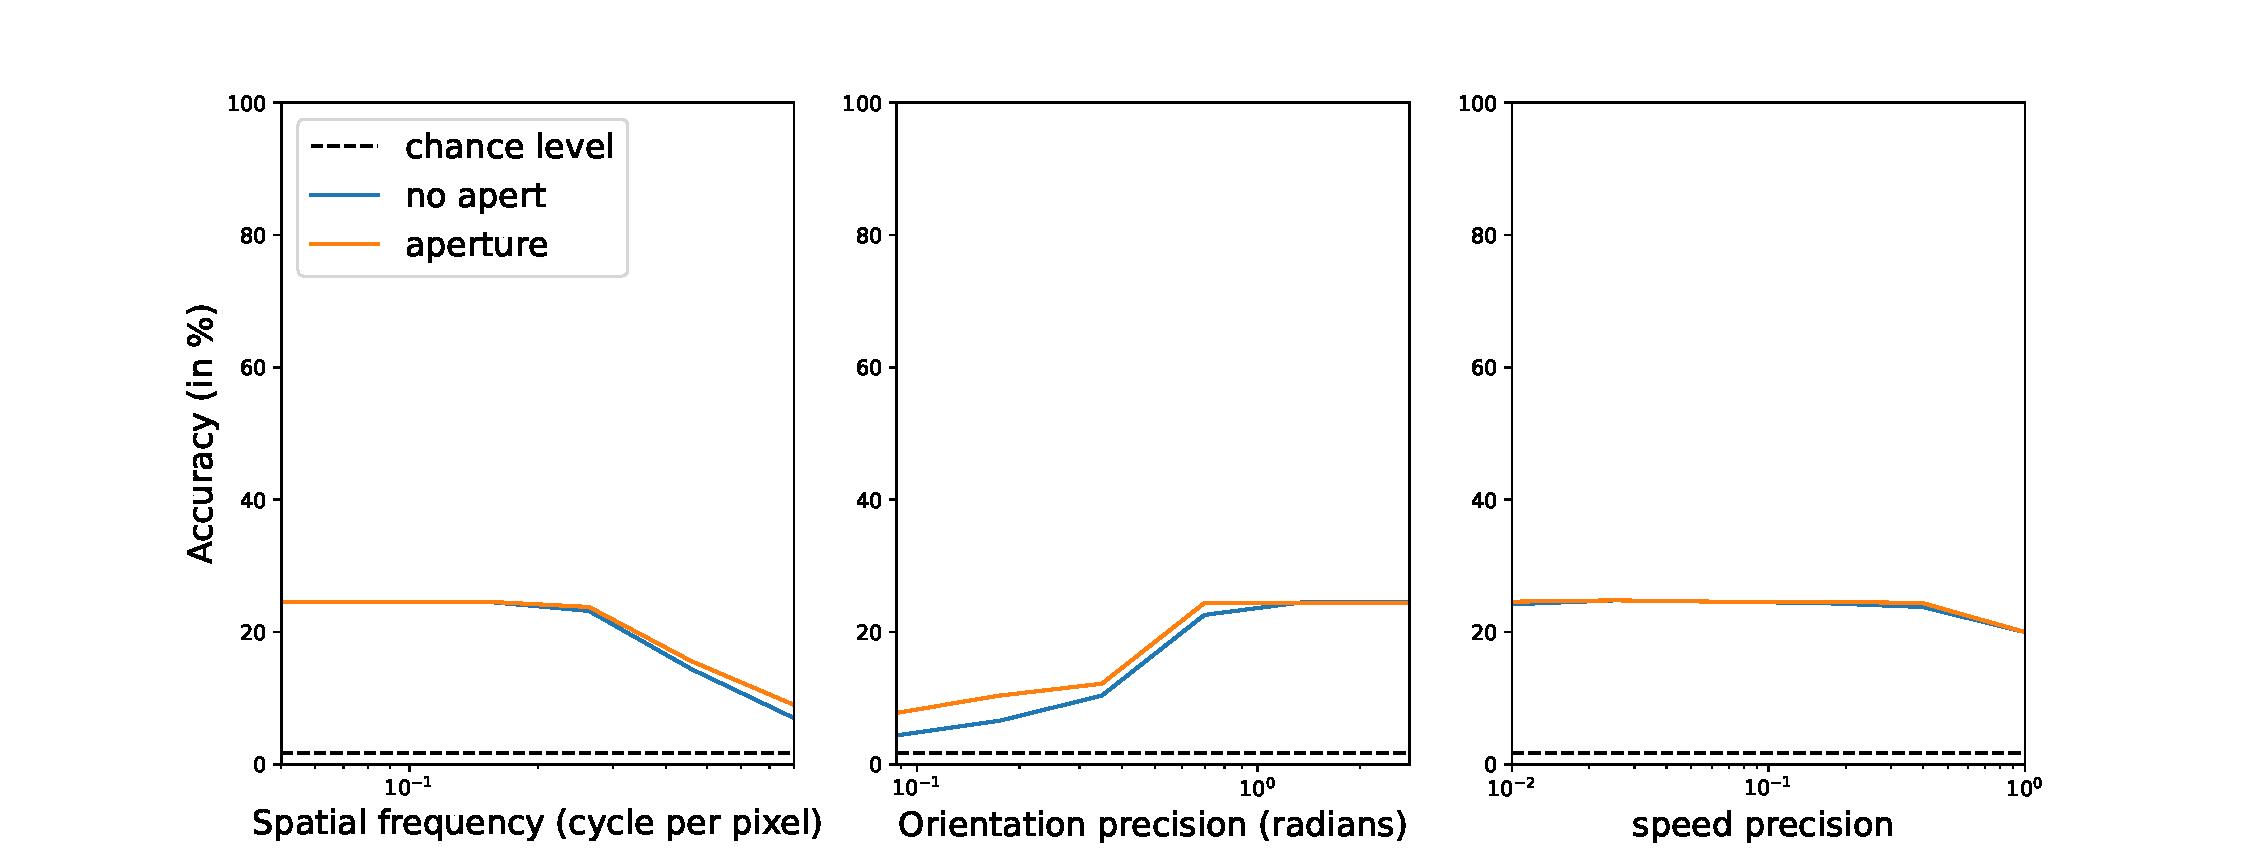
\includegraphics[width=0.95\linewidth]{figures/motion_clouds.pdf}
    \caption{{\bf Role of stimulus parameters in the motion detection accuracy.} Accuracy as a function of {\bf (a)} the mean spatial frequency, {\bf (b)} the bandwidth in orientation: from a grating-like (left) to isotropic textures (right)), {\bf (c)} the bandwidth in speed, from a rigid motion (left) to independent frames (right). Note that these accuracy is computed both in the case is necessarily perpendicular to the motion (no aperture) or arbitrary (aperture), showing that accuracy decreases in the latter case.}
    \label{fig:motion_clouds}
\end{figure}
%%%-----------------------------------------------------------------

We plot here main axis of interests. First, as we change the mean spatial frequency of the texture, we observe a monotonous decrease in accuracy. This comes as a similar trend as that observed in the primary visual areas~\citep{priebe_tuning_2006}. \note{we should really do something more serious here...} Notably, the accuracy is better for a large spatial frequency bandwidth (which qualitatively resemble a more textured stimulus) than for a grating-like stimulation, reminiscent to the behavioral response of humans' eye movements to such stimuli~\citep{simoncini_more_2012}. Interestingly, we also see a modulation of accuracy as a function of orientation bandwidth. When the stimulus is grating-like and that the orientation is arbitrary with respect to the direction of motion, the system is faced with the aperture problem and see a decrease of accuracy. This is not the case for isotropic stimuli or when the orientation is perpendicular to the direction of motion. Finally, we manipulated the amount of change between two successive frames, similar to a temperature parameter. This shows a progressive decrease in accuracy, similar to that observed in the amplitude of humans' eye movements~\citep{mansour_pour_speed_2018} but also that accuracy is low for a rigid motion which lacks variability.
%
\subsection{Accuracy for the motion detection task}
%%%-----------------------------------------------------------------

Once our MLR is trained, we obtain spatio-temporal kernels corresponding to the weights associated to the heterogeneous delays of our layer of spiking neurons and which may be used for detection. We observed that the distribution of the kernels' weights is sparse, with most values near zero. As shown in the formalization of our event-based model, the computational cost of our model if implemented on a neuromorphic chip would be dominated by the number of spikes times the number of synapses. Indeed, the computations are dominated by the convolution operation. In a dense setting, this corresponds for all voxels in the output to a sum over all voxels in the inputs for all weights in the kernel. If the support of information is sparse, then computations can be performed only on those events. Also, if we set some weights of the kernels to zero, then the sum can be skipped for those addresses. Knowing the sparseness of the input, the total number of computations thus scales with the number of nonzero synaptic weights. 

To assess the robustness of the classification as a function of the computational load, we will prune the weights in $\{\synapse_\ranksyn\}_{\ranksyn \in [0,\Nsyn)}$ that are below a defined threshold. In Figure~\ref{fig:accuracy}, we plot the classification accuracy as a function of the relative number of computations, or active weights, per decision for each neuron of the layer. As a comparison and to account for the gain in performance by using heterogeneous delays, we provide the accuracy obtained with a MLR model using 2D time surface (in red) as in~\citep{grimaldi_robust_2022}. This latter method is based on delays from the last recorded events and uses fewer computations (in our case $15\times15$) than the dense 3D kernels without any pruning ($15\times15\times8$). While less computations are needed, the classification performance obtained for the model using time surfaces is similar to our method using all the weights of the kernels.

By pruning weights, we observe that the evolution of accuracy as a function of the log percentage of active weights fits well a sigmoid curve. Half-saturation level is reached at about $3.5\times 10^{-3}\%$ of active weights, corresponding in our setting to a total amount of $6$ computations per decision. Compared to the full kernels, the accuracy of our method is maintained to its top performances when dividing the number of computations by a factor up to about $200$. In this case, the number of computations is greatly reduced compared to~\citep{grimaldi_robust_2022}, thus demonstrating the efficiency of the presented method. 

%
%%%-----------------------------------------------------------------
%: fig:accuracy
%%%-----------------------------------------------------------------
\begin{figure}%[h!]
    \centering
    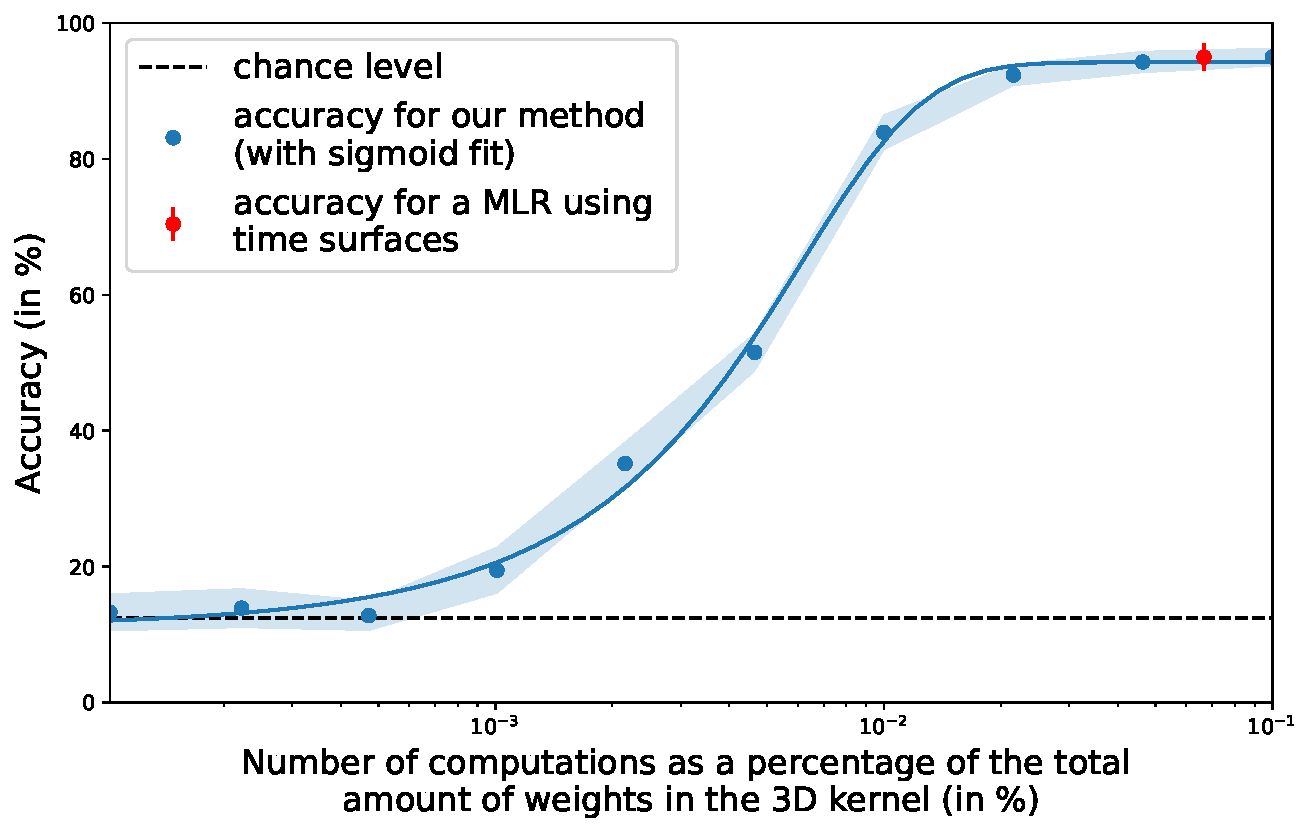
\includegraphics[width=0.95\linewidth]{figures/accuracy.pdf}
    \caption{Accuracy as a function of the number of computation load for the heterogeneous delays model (blue line) and for a method using 2D time surfaces (red dot)~\citep{grimaldi_robust_2022}. The relative computational load (on a log axis) is controlled by changing the percentage of active weights relative to the dense convolution kernel. We observe a similar accuracy than HOTS, yet that our model could achieve a similar accuracy with significantly fewer coefficients.}
    \label{fig:accuracy}
\end{figure}

\note{try also a quantization of the weights (binary?)}
%
\section{Discussion}
%%%-----------------------------------------------------------------
%%%-----------------------------------------------------------------
In this paper, we have introduced a generic SNN using heterogeneous delays and have shown how it compares favorably for a visual motion detection task with a state-of-the-art event-based algorithm used for classification. The learned model bears many similarities with neurobiological anatomical observations but also with the results from behavioral results. \note{to change if we compare to ghosh instead of HOTs if we follow that route} The event-driven computations of our method can be reduced drastically through the pruning of synapses, while maintaining top performance for classification. This shows that we may use the precise timing of spikes to enhance neural computations. 
%
\subsection{Synthesis and main contributions}
%%%-----------------------------------------------------------------
To recap, we have introduced in this paper a SNN model with heterogeneous delays that we have trained and evaluated on a complex motion detection task. The model was defined to optimally detect event-driven spatio-temporal motifs. We have shown that when the model is trained on a dataset of natural images with realistic eye movements, the model learns kernels similar to those found in the early visual cortex of humans for example. We have then shown that the model displays similarities with the responses observed in biology. We have evaluated the computational cost of this model if implemented on neuromorphic hardware, showing that the use of heterogeneous delays may be a frugal computational solution for future neuromorphic hardware, but also a key to understand why spikes represent a universal component of neuronal information processing.

Let us highlight some innovations in the contributions presented in this paper. First, the generic heterogeneous model is formalized from first principles for optimal detection of the event-based spatio-temporal motifs, whereas~\citet{ghosh_spatiotemporal_2019,yu_stsc-snn_2022} use a correlation-based heuristic, which we have observed to be less efficient. Moreover, in comparison to HOTS~\citep{lagorce_hots_2017} the weights are explainable as they directly inform on the logit (inverse sigmoid of the probability) of detecting each spatio-temporal spiking motif. Another novelty is that the model simultaneously learns the weights and the delays, while for example the polychronization model~\citep{izhikevich_polychronization_2006} only learns the weights using STDP while the delays are randomly drawn and their values frozen. Moreover, the model is evaluated on a realistic task, while models such as the tempotron are tested on simplified problems~\citep{gutig_tempotron_2006}. Another main contribution is to provide a model that is suitable for learning any type of spatio-temporal spiking motifs and that can be trained in a supervised way by providing a dataset of supervision pairs. This allows for a more flexible definition of the model using this properly labeled dataset instead of relying on a careful description of the physical rules governing a task, e.g., the luminance conservation principle for motion detection~\citep{benosman_asynchronous_2012, dardelet_event-by-event_2021}.
%
\subsection{Main limits}
%%%-----------------------------------------------------------------
We have identified several limits to our model, which we will now detail. First, the complete framework is based on a discrete binning of time that is incompatible with the continuous nature of biological time. We have used this binning to be able to efficiently implement the framework on conventional hardware, especially GPUs, and in particular to be able to use three-dimensional convolutions. We have tested the effect of the size of the time bin and shown that it has essentially no impact on the results presented in this paper. This is consistent with the relative robustness of other event-based frameworks such as HOTS~\citep{lagorce_hots_2017}, where the accuracy was not affected when the input spikes were subjected to noisy perturbations up to $1~\ms$~\citep{grimaldi_robust_2022}. This suggests the possibility of analytically including a precision term in the temporal value of the input spikes, a mechanism potentially implemented by the filtering that is implemented by the synaptic time constant of about $5~\ms$. Furthermore, it is possible to circonvent the necessity of using a time discretization by using a purely event-based scheme. Indeed, it is not necessary to compute voltage traces between two spikes~\citep{hanuschkin_general_2010} and it is thus possible to define a purely event-based framework. Such an architecture could provide promising speed gains for the calculations.  \note{pourrait parler du poster bernstein? de nadafian?}

Another restriction is that this model is purely feed-forward. Therefore, the spikes generated by the postsynaptic neurons are produced solely on the basis of information contained in the classical receptive field. However, it is well known that neurons in a layer can interact using lateral interactions, for instance in V1 and that this can be the basis for computational principles~\citep{chavane_revisiting_2022}. For example, the combination of neighboring orientations may contribute to image categorization~\citep{perrinet_edge_2015}. Furthermore, neural information is modulated by feedback information, for example to distinguish a figure from its background~\citep{roelfsema_early_2016} and it has been shown that feedback may be essential for building realistic models of primary visual areas~\citep{boutin_sparse_2020, boutin_effect_2020}, Notably to explain non-linear mechanisms~\citep{boutin_pooling_2022}. It is currently not possible to implement these recurrent connections in our implementation (lateral or feedback), mainly due to our use of convolutions. However, the generic theoretical model is able to include them by inserting new spikes into the list of spikes that are reaching pre-synaptic addresses. While this is possible in theory, it needs to be properly adapted in practice so that these recurrent connections do not amplify neuronal activity outside a homeostatic state (through an extinction or explosion of activity).  
\note{ dire que la prédiction permet de faire de la prediction et que ça explique les résultats de leBec}%~\citep{perrinet_motion-based_2012}


Such recurrent activity would be essential for implementing predictive or anticipatory processes. This is essential in a neural system, as it contains multiple different delays that require temporal alignment~\citep{hogendoorn_predictive_2019}. This has been previously modeled to explain for example the flash-lag illusion~\citep{khoei_flash-lag_2017}. \note{Say that this could be implemented by properly setting the timing of the label} As previously stated, this could be implemented using generalized coordinates (that is variables such as position which are complemented by speed, acceleration, jerk, ...) and ``neurobiologically, the application of delay operators just means changing synaptic connection strengths to take different mixtures of generalized sensations and their prediction errors''~\citep{perrinet_active_2014}. Our proposed model using heterogeneous delays provides an alternate and elegant implementation solution to this problem.
%
\subsection{Perspectives}
%%%-----------------------------------------------------------------
\note{la tache ne met pas en avant les capacites des motifs hetero synaptiques =trop simple et peut se faire en HOTS}
In the definition of our task, we highlighted how the generation of events depends on the spatial gradient in each image. This gradient is defined in both horizontal and vertical dimensions and its maxima are generally oriented. Taken together, these oriented edges form the contours of visual objects in the scene~\citep{koenderink_representation_1987}. Thus, there is a dependence within the event stream between motion and orientation information. It would be crucial to study this interdependence further. This could be initiated by training the model on a dataset with labels providing local orientation. \note{we can say we tried and that it works well}. Studying this dependence will allow us to dissociate these two forms of visual information and to enable us to integrate them. In particular, it will allow us to consider that the definition of motion is more accurate perpendicular to an oriented contour (aka, the aperture problem), thus allowing us to implement recurrent predictive rules, such as those identified to dissociate this problem~\citep{perrinet_motion-based_2012}.

The model is trained on a low-level local motion detection task, and one might wonder if it could be trained on higher-level tasks. An example task would be depth estimation in the visual scene. There are multiple sources of information for inferring depth, such as binocular disparity or changes in texture or shading, but in our case, motion parallax would be the most significant cue~\citep{rogers_motion_1979}. This is because objects close to an observer move relatively faster on the retina than an object at a great distance, and also that visual occlusions depend on depth ordering. Using this information, one can segment objects and estimate their depth~\citep{yoonessi_contribution_2011}. However, this would require computing first the optical flow, that is extending the framework described here for a rigid full-field motion to a more generic one where motion may vary in the visual field. A possible implementation is therefore to add a new layer to our model, in analogy with the hierarchical organization highlighted in the visual cortex. This is theoretically possible by using the output of our model (which estimates velocity in retinotopic space) as input to a new layer of neurons that would estimate velocity in the visual field, including the depth dimension in the output supervision labels. This could have direct and important applications, for example in autonomous driving, to detect obstacles in a fast and robust way. Another extension would be to actively generate sensor movements (physically or virtually) to yield better depths estimates, notably to disambiguate uncertain estimates~\citep{nawrot_eye_2003}.

In conclusion, the model we have presented provides a way to efficiently process event-based signals. We have shown that we can train the model in a semi-supervised manner, knowing \emph{what} output label but not knowing \emph{when} it occurs. Another perspective would be to extend the model to a fully self-supervised learning paradigm, i.e., without any labeled data~\citep{barlow_unsupervised_1989}. This type of learning is thought to be predominant in the central nervous system and, assuming that the signal is sparse~\citep{olshausen_emergence_1996}, one could extend those Hebbian sparse learning schemes to spikes~\citep{perrinet_emergence_2004, masquelier_competitive_2009}. We anticipate that this would be particularly well suited to the exploration of neurobiological data. In fact, there is a substantial literature indicating that brain dynamics often organize into stereotyped sequences such as synfire chains~\citep{ikegaya_synfire_2004}, packets~\citep{luczak_sequential_2007}, or hippocampal sequences~\citep{pastalkova_internally_2008, villette_internally_2015}. These motifs are stereotypical and robust, as they can be activated in the same motif from day to day~\citep{haimerl_internal_2019}. In contrast to conventional methodologies that are used to process neurobiological data, such a event-based model would be able to answer key questions regarding the representation of information in neurobiological data. Furthermore, it would open up possibilities in the field of machine learning, especially in computer vision, to address current key concerns such as robustness to attacks, scalability, interpretability, or energy consumption.
%
%%%%%%%%%%%%%%%%%%%%%%%%
\backmatter
%
\bmhead{Acknowledgments}
%
% Acknowledgement hidden for review.
\Acknowledgments
%
%%%%%%%%%%%%%%%%%%%%%%%%

\section*{Statements and Declarations}

\paragraph{Funding}

\Funding %

\paragraph{Conflict of interest}
Not applicable.
% The authors do not have any financial or non-financial interests directly or indirectly related to this work.

\paragraph{Ethics approval}
Not applicable.

\paragraph{Consent to participate}
Not applicable.

\paragraph{Consent for publication}
Not applicable.

\paragraph{Availability of data and materials}
Not applicable.

\paragraph{Code availability}

The code is publicly available online at: \url{https://github.com/SpikeAI/pyTERtorch}.

\paragraph{Authors' contributions}

Both authors contributed to the conceptualization and methodology design of the study, to the project's coordination and administration. Laurent Perrinet carried out the funding acquisition and supervision. Formal analysis and investigation were performed by both authors. Results visualization and presentation were realized by both authors. The the manuscript was written by Laurent Perrinet. Both authors have read and approved the final manuscript.
%%%%%%%%%%%%%%%%%%%%%%%%
\bibliographystyle{apalike}
\bibliography{FastMotionDetection}
\end{document}
%%%%%%%%%%%%%%%%%%%%%%%%